\cotefile{156-6}
\scanpage{88}\mspage{87}

\uline{At \deleted{\unsure{14 bis}}(\unsure{fac|Fac}) 14 bis} Sous les conditions précédentes, \deleted{\unsure{considérons}} considérons
\deleted{\unsure{Mettons le|tel que le|tels que le}}
\diagram{\begin{tikzcd}[ampersand replacement=\&, column sep=.3em,row sep=1.3em]
\widetilde G \& \subset \& \widetilde F \\
\widetilde G' \arrow[u] \& \&
\end{tikzcd}}
alors on peut trouver $F'\preccurlyeq F$ induisant $G'$, de telle façon que dans le diagramme d'ens \inserted{ordonnés}
\diagram{\begin{tikzcd}[ampersand replacement=\&,column sep=2.6em,row sep=2.6em]
\widetilde G'_{\deleted{\unsure{t|+}}} \arrow[r,hook] \arrow[d,"{\varphi\mathbin{\unsure{\vert}}\widetilde G'}"'] \arrow[dr,phantom,"\text{\unsure{cart}}" description] \& \widetilde F' \arrow[d,"\varphi"]\\
\underset{\substack{\text{\unsure{sous ens.}}\\\text{fermé}}}{\widetilde G} \arrow[r,hook] \& \widetilde F
\end{tikzcd}}
on ait $\widetilde F'\setminus\widetilde G'_{t}\overset{\substack{\text{iso d'ens.}\\\text{ordonnés}}}{\xrightarrow{\sim}}\widetilde F\setminus\widetilde G$, et pour $\xi\in\widetilde G'_{t}$, $\eta\in\widetilde F'$, on ait $\xi\leq\eta$ \unsure{sss|ssi} $\varphi^{\unsure{\#|*}}(\unsure{\vert|\xi})\leq\varphi^{\#}(\eta)$.

[ce qui détermine l'ens. ordonné $\widetilde F'$ et le diagramme précé\uline{dent,} à iso unique près].

\margin{\uline{22. juin}}Je présume qu'on doit pouvoir prouver qu'un tel $F'$ est unique, comme la plus grande des subdivisions de $F$ induisant $G'$ sur $G$.\margin{\unsure{unicité automatique} ???}% slanted
 Dans \unsure{les|le} cas où $\unsure{\mathcal F|\exists}$ est à figures finies (pour \unsure{éviter|iviter} des inductions transfinies \ldots), \deleted{cette} condition doit être équivalente à

\noindent\begin{tabular}{@{}||p{.90\linewidth}@{}}
At (fac) 14 ter : Soit $X\in M$, et $F'\preccurlyeq\partial X$. Alors il existe un unique $X'\in M$ tel que $X'\preccurlyeq X$, $\partial X'=F'$
\end{tabular}
\scanpage{89}\mspage{88}

Nous imposerons \unsure{du moins|de même} cette condition pour les ateliers \uline{saturés} (cf plus bas). Mais on notera que cette condition n\deleted{\unsure{'est}}e sera pas vérifiée dans \unsure{les|le} cas d'ateliers \deleted{\unsure{semi}} simpliciaux \inserted{\unsure{stricts|strict}}, par exemple
\figure{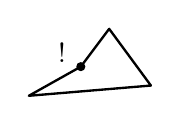
\begin{tikzpicture}[x=1cm,y=1cm,line join=round]
\draw[line width=.85pt] (0,0) -- (.66,.37) -- (1.02,.85) -- (1.55,.13) -- cycle;
\fill (.66,.37) circle[radius=1.65pt];
\node at (.42,.54) {$!$};
\end{tikzpicture}}
est un contre-exemple.

(Atelier simplicial : tout $X\in M$ est un ``simplexe combinatoire'', ou encore : \inserted{$\forall X\in M$,} \deleted{\unsure{toute}} partie \deleted{majorée} \inserted{non vide} de $\deleted{\unsure{M}}{\widetilde X}$ \inserted{(pour $\leq$)} \unsure{a} un sup, \inserted{\unsure{tout} élément non minimal a au moins \unsure{deux} prédécesseurs, $\unsure{\#|*}$} \deleted{\unsure{les}} et $\widetilde X$ \deleted{\unsure{sont}} \unsure{fini|finis}, \deleted{Attention \unsure{;|:} se \unsure{faut-il|peut-il} que tout \unsure{élém.} non minimal a au \unsure{moins} \unsure{deux} préd.} \deleted{toute partie finie \inserted{\unsure{non vide} majorée} de $M$ a un sup, et les $\widetilde X$ sont finis.]} pas que toute partie finie \unsure{majorée} de $M$ ait un sup, \unsure{(}ex :
\figure{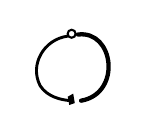
\begin{tikzpicture}[x=1cm,y=1cm,line cap=round]
\draw[line width=1.05pt] (.39,.86) .. controls (.09,.82) and (-.10,.50) .. (.04,.23) .. controls (.13,.09) and (.30,.05) .. (.43,.04);
\draw[line width=1.55pt] (.52,.88) .. controls (.98,.94) and (1.08,.13) .. (.56,.04);
\draw[fill=white,line width=.75pt] (.44,.89) circle[radius=1.45pt];
\fill (.41,-.015) -- (.48,.01) -- (.46,.13) -- (.39,.09) -- cycle;
\end{tikzpicture}}
)
\margin{Atelier simplicial strict : simplicial et $X\unsure{\mathrel{\mathord{\rlap{$>$}<}}|,|\mathrel{\lesseqgtr}}Y$ \unsure{compatible|compatibles} $\Longrightarrow X\cap Y$ \inserted{\unsure{ens}} $\in M$ i.e. : Si $\{X,Y\}$ \deleted{\unsure{vide}} \inserted{\unsure{minorée|minoré}}, $\unsure{\inf|\mathrm{Inf}}(X\unsure{.|,}Y)$ existe dans $M$}% slanted

Pour le moment, je voudrais

1$^\circ$) Expliciter les axiomes dans le cas d'un atelier ensembliste

2$^\circ$) Voir leur stabilité ou non stabilité par passage à un sous-atelier

3$^\circ$) Étudier l'opération de \uline{saturation} d'un atelier (en me restreignant au besoin au cas d'un atelier ``modéré'').

Nous avons vu (p. \unsure{55-53|55-57|56-53|55-55}) qu'un atelier ensembliste est défini par un ens $L$ et une partie \deleted{$\unsure{\mathcal F\subset|\mathcal F\in}$}
\[
\mathcal F\subset\mathrm{Fig}(L)
\]
satisfaisant les conditions $\unsure{\mathrm{At}\,\mathrm{ens}^{\alpha}|\mathrm{At}\,\mathrm{ens}^{a}}$ 1, 2, 3.

$\unsure{\hookrightarrow|G|\subset}$ On a déjà vu qu'on a alors automatiquement At 1 à At 8. Il faut examiner les autres axiomes. Pour les exemples et contre exemples on pensera surtout au cas $L$ fini, et où on \inserted{peut se reporter au point de}
\scanpage{90}\mspage{89}

\deleted{At 9 \unsure{Je pense notamment au cas}}

vue d'une donnée de $M$ ens de figures él. dans $L$, avec relation $\mathrel{\underset{\unsure{M|\mu}}{\mathord{\rlap{$>$}<}}}$, satisfaisant At ens \unsure{tf|If|lf|H} 1 -- At ens tf 3. Si on prend p. ex
\[
M=\Bigl\{\{\{x\}\unsure{\}|\{}{\deleted{\unsure{\}}}}_{\deleted{x\in L}}\mid x\in L\deleted{\unsure{\}}}\Bigr\},
\]
alors la donnée \unsure{est} \unsure{restreinte|exactement|revient} à celle d'une relation \inserted{\unsure{sym. refl.}} $x\mathrel{\underset{\deleted{\unsure{M}}}{\mathord{\rlap{$>$}<}}}y$ \uline{dans $L$}. (les conditions At ens tf 1--3 étant trivialement satisfaites).

At 9 dans ce cas-là \deleted{signifie que} \inserted{est vérifié \inserted{automatiquement}}. Dans \deleted{\unsure{le|du}} cas général, il se traduit par

\deleted{\unsure{At ens} $ {\unsure{9}}^{*}$ \unsure{4}}

\deleted{\uline{\unsure{At ens tf}} \unsure{4}}

\[
\begin{aligned}
&\text{Si } X,Y\in M \text{ et } \inserted{|X|\cap|Y|=\varnothing.\ \text{Alors }X\mathrel{\underset{M}{\mathord{\rlap{$>$}<}}}Y\ \text{\unsure{sss|ssi}}}\ \forall x\in|X|,\,y\in|Y|,\\
&x\mathrel{\underset{M}{\mathord{\rlap{$>$}<}}}y,\quad \deleted{\unsure{\text{alors }X}}
\end{aligned}
\tag*{($*$)}
\]

Mais compte tenu de \uline{Atens} 2, cela équivaut à

\uline{Atens} 2 (ou Atens tf 4) Si $X,Y\in M$ et $|X|\cap|Y|=\varnothing$, alors $X\mathrel{\underset{M}{\mathord{\rlap{$>$}<}}}Y$ (\deleted{\unsure{donc}} $X\parallel Y$)
\margin{\textendash\quad En fait, on aura donc $X\parallel Y$ sss $|X|\cap|Y|=\varnothing$}% slanted

At ens $9_{\Sigma}$ se traduit par

\uline{Atens} $\deleted{\unsure{2}}{\unsure{3|2}}_{\Sigma}$ (ou Atens tf $4_{\Sigma}$\unsure{]|)} \deleted{Soient} $X,Y\in M$,

\noindent\begin{tabular}{@{}|p{.91\linewidth}@{}}
soit $K$ l'ens des strates communes à $X$ et $Y$ \inserted{(qui est \unsure{la|$C$|$\in$} \unsure{fig ens. ind.})}.

Pour que $X\mathrel{\underset{M}{\mathord{\rlap{$>$}<}}}Y$, il \unsure{f} et s que $|X|\cap|Y|=K$ \deleted{\unsure{et}} (i.e. $X\mathrel{\underset{\mathrm{ens}}{\mathord{\rlap{$>$}<}}}Y$) \uline{et} $K\in\Sigma$.
\end{tabular}
\scanpage{91}\mspage{90}

Le cas où $\Sigma=$ tous les ens. ordonnés (axiome At $9'$) ceci équivaut à dire que $\mathcal F$ est un sous-atelier \uline{spacieux} de \deleted{$\unsure{\mathcal F|\Sigma}$} $\mathrm{Fig}(L)$\unsure{,|.} Mais \deleted{\unsure{de}} on se rappellera que ce ne sera pratiquement jamais le cas pour les ateliers \deleted{\unsure{semi|stricts}} simpliciaux.

At 10 automatique par At ens (2).

\uline{At \deleted{\unsure{11 bis|11}}ens 3} Axiome de stabilité par Sup. filtrantes $\operatorname{Sup} F'_i$, quand les $F_i\ll F$ et la famille $F_i$ est ``loc$^{\mathrm t}$ finie \unsure{p.r.} à $F$''.
\margin{va dans la \unsure{direction} ``très spacieux''\ldots}% slanted

Cet axiome est vide dans le cas où les figures $\in\mathcal F$ sont \deleted{\unsure{de st.f. finie|de st.f. fini}} de \unsure{t.f.|tf.}. (\unsure{car} alors la famille $({\unsure{\mathbb F|\mathcal F|F}}'_i)$ sera \unsure{alors|elle} $=$ \unsure{stationnaire} \ldots)

\inserted{At \deleted{\unsure{ens}} 12 (en l'absence de At \deleted{\unsure{ens}} $9_{\Sigma}$ i.e. Atens $2_{\Sigma}$) donne}

\uline{At ens \deleted{\unsure{5}}4} (ou At ens \unsure{tf|If|lf|H}. \deleted{\unsure{4}}$\unsure{5|4}$) Soient \deleted{$X,Y\in M$,} $X'\ll X$; $Y'\ll Y$ dans $M$, \deleted{$K=X\unsure{,|\cap}Y$} avec $X\mathrel{\underset{\unsure{M|\mu}}{\mathord{\rlap{$>$}<}}}Y$, $K=X\cap Y$. Si $X'_{K}\mathrel{\underset{M}{\mathord{\rlap{$>$}<}}}Y'_{K}$ (i.e. pour \unsure{tt|tte|toute} \deleted{\unsure{x}} $X''\in\widetilde X'$ telle que $X''\deleted{\unsure{\ll|\leq}}\ll\deleted{\unsure{Y}}K$ (\unsure{i.e.|i.e} $ {\unsure{A|X}}''\ll Y$) toute $Y''\in\widetilde Y'$ telle que $Y''\ll K$ (i.e $Y''\ll X$) on a $X''\mathrel{\underset{M}{\mathord{\rlap{$>$}<}}}Y''$, alors $X\mathrel{\underset{M}{\mathord{\rlap{$>$}<}}}Y$.
\margin{Résulte de Atens $2_{\Sigma}$}% slanted

Grâce à At ens 2, on voit que \deleted{\unsure{At}} la condition sur $F\ll\deleted{\unsure{O}}X$ dans At 13 signifie \unsure{par|que} $|F|\subsetneq|X|$, et \deleted{que} que At 13 est toujours vérifié.
\scanpage{92}\mspage{91}

La condition At 14 (peut-être \unsure{facultative}) semble \deleted{plus} un peu \unsure{abracadabrant|abracadabrante}, traduite en termes de \unsure{sous-atelier|sous-ateliers} d'un $\mathrm{Fig}(\mathscr L)$ -- ce n'est plus dans la nature d'une condition de stabilité.

De ce point de vue, l'axiome At 14 bis \unsure{``|``(}facultatif) est plus sympathique :

\uline{At ens fac} 5 : Soit $X\in M$, et $F'\preccurlyeq\partial X$

\noindent\begin{tabular}{@{}||p{.90\linewidth}@{}}
avec $ {\unsure{\mathbb F|F}}'\in M$. Considérons \unsure{l'unique|le 'unique} figure \deleted{\unsure{en}} $F\in\mathrm{Fig}(L)$ qui soit élémentaire et telle que $\partial F=F'$. Alors $F\in M$.
\end{tabular}

Mais ce sera pas vrai pour les ateliers simpliciaux !

\begin{center}\rule{1.7cm}{.35pt}\end{center}

Passons à la situation d'un atelier $\mathcal F$, et d'un sous-atelier $\mathcal F'\subset\mathcal F$.

(cf conditions Sous at 1, 2 p. \unsure{47|41})

Les conditions At 1 à At 7 sur \deleted{\unsure{tout|tous}} $\mathcal F$ se transportent aussitôt à $\mathcal F'$.

Pour les conditions impliquant $L$ (At 8, 9, $9_{\Sigma}$, 10) il faut déjà pouvoir comparer $\deleted{\mathcal F}\unsure{L|\mathscr L}$ et $\deleted{\mathcal F'}L'$. \unsure{Èvidemment|Évidemment} \deleted{$\unsure{L}$}
\[
L\cap\mathcal F'\subset L'
\]
\scanpage{93}
\mspage{92}

on voudrait que l'on ait égalité, i.e. que tout \unsure{élémt|élément} minimal de $\deleted{\unsure{\Delta|\mathcal F}}\mathcal F'\setminus\{\unsure{\phi|\varnothing}\}$ \inserted{pour $\ll$} appartienne à $\mathcal F$. On posera

\uline{Définition} On dit que le sous-atelier $\mathcal F'$ de $\mathcal F$ est \uline{épais} (pour les lieux) si $F\unsure{\in|\subseteq}\mathcal F'\Rightarrow\unsure{\mathrm{omb}|\mathrm{amb}}(F)\subset\mathcal F'$ i.e. \unsure{.}$F\in\mathcal F',\ x\ll F\quad(x\in L)\Rightarrow x\in\mathcal F'$. Il est dit \deleted{\unsure{quasi|quas}} \unsure{quasi-dense} si \inserted{$\forall X\in M'=\mathcal F'\cap M,\ \exists x\in L\cap\mathcal F'$ avec $x\overset{\circ}{\ll}X$ \inserted{i.e. $x\in\mathrm{omb}(X)^\circ$}} Cela équivaut à

\unsure{``}\uline{Sous at} (\deleted{\unsure{plein}}\unsure{épais}) 3 $\forall X\in\deleted{\unsure{\mathcal F|F}}M',\ x\in L,$ t.q. $x\ll X,$
\[
x\in\mathcal F'.
\]
\margin{\unsure{$T$|$J$} \unsure{$-$}}

\deleted{Ceci dit} ou

\deleted{\uline{Corollaire}}

\uline{Sous-at} (qu. \unsure{dense|den}) $3'$ $\forall X\in M'=\mathcal F'\cap M,\ \exists x\in L\cap\mathcal F'$ avec $x\overset{\circ}{\ll} X$

Bien sûr, Sous at $3\to$ Sous at $3'$ et ce dernier implique At 8 pour $\mathcal F'$, \deleted{\unsure{ce} \illegible{2}} le \unsure{premier} implique d'ailleurs
\[
L'=L\cap\mathcal F'\qquad .
\]

Ceci dit, At 9 n'est pas néc. stable par passage à \unsure{``}sous-atelier, même plein. Pour être content, on voudra

% slanted
\margin{dans la nature \unsure{d'une|des images} \unsure{exprime|a priori|séparation} \unsure{aussi} ``\unsure{propriété|propreté}}
\uline{Sous-at} 4 Si $X,Y\in M'$ et $X\parallel Y$ dans $\mathcal F$, alors $X\parallel Y$ dans $ {\unsure{\mathcal F|\mathbb F}}'$ ($\Longleftrightarrow X\mathrel{\underset{\mathcal F'}{\mathord{\rlap{$>$}<}}}Y$)
\scanpage{94}
\mspage{93}

qui va impliquer, \deleted{\unsure{pour|que} \unsure{si}} avec Sous-at 3 (atelier plein) que si $\mathcal F$ satisfait At 9, $\mathcal F'$ aussi (\unsure{sans} que dans Sous at 4 il soit question des lieux).

Moyennant Sous at 4, \deleted{\unsure{At|4}} \inserted{et Sous at 3} At 10 pour $\mathcal F'$ implique \deleted{\unsure{que|pour}} \unsure{itou|item} pour $\mathcal F$.

At 11 bis \inserted{(\unsure{ou|en} At 11)} pour $\mathcal F'$ est une propriété de stabilité \inserted{de $\mathcal F'$ dans $\mathcal F$}, \unsure{nullement|nullmt} automatique. Idem pour At 12. Pour At 13, \deleted{\unsure{dans|de}} moyennant Sous at 3, Sous at 4, sa validité dans $\mathcal F$ l'implique dans $\mathcal F'$

At 14 est \unsure{abracadabra-|abracadabra|abracadabran}, At 14 bis dans la nature d'une condition de stabilité.

\begin{center}
\rule{1.35em}{0.4pt}
\end{center}
